% !TEX encoding = UTF-8 Unicode
% !TEX root = ../thesis.tex
\chapter{Introducción} \label{intro}
Este es un capítulo de ejemplo.
\section{Configuración de Página}
Los siguientes son los parámetros de configuración de la página de este formato en latex.
\pagevalues

Esto que sigue es un footnote: %\footnote{footnote number 1 working fine}
%
\begin{figure}
	\pagediagram
	\caption{Diagrama de página}
	\label{fig1_intro}
\end{figure}

La Fig. \ref{fig1_intro} muestra el formato que adopta Latex para el Layout.

Como se puede apreciar en la Fig. \ref{fig2_intro}, los lápices tienen muchos colores, los mismos se pueden generar de diversas formas \cite{ejemplo}.

Las referencias pueden ser en formato APA o IEEE.

\begin{figure}[htb]
	\centering
	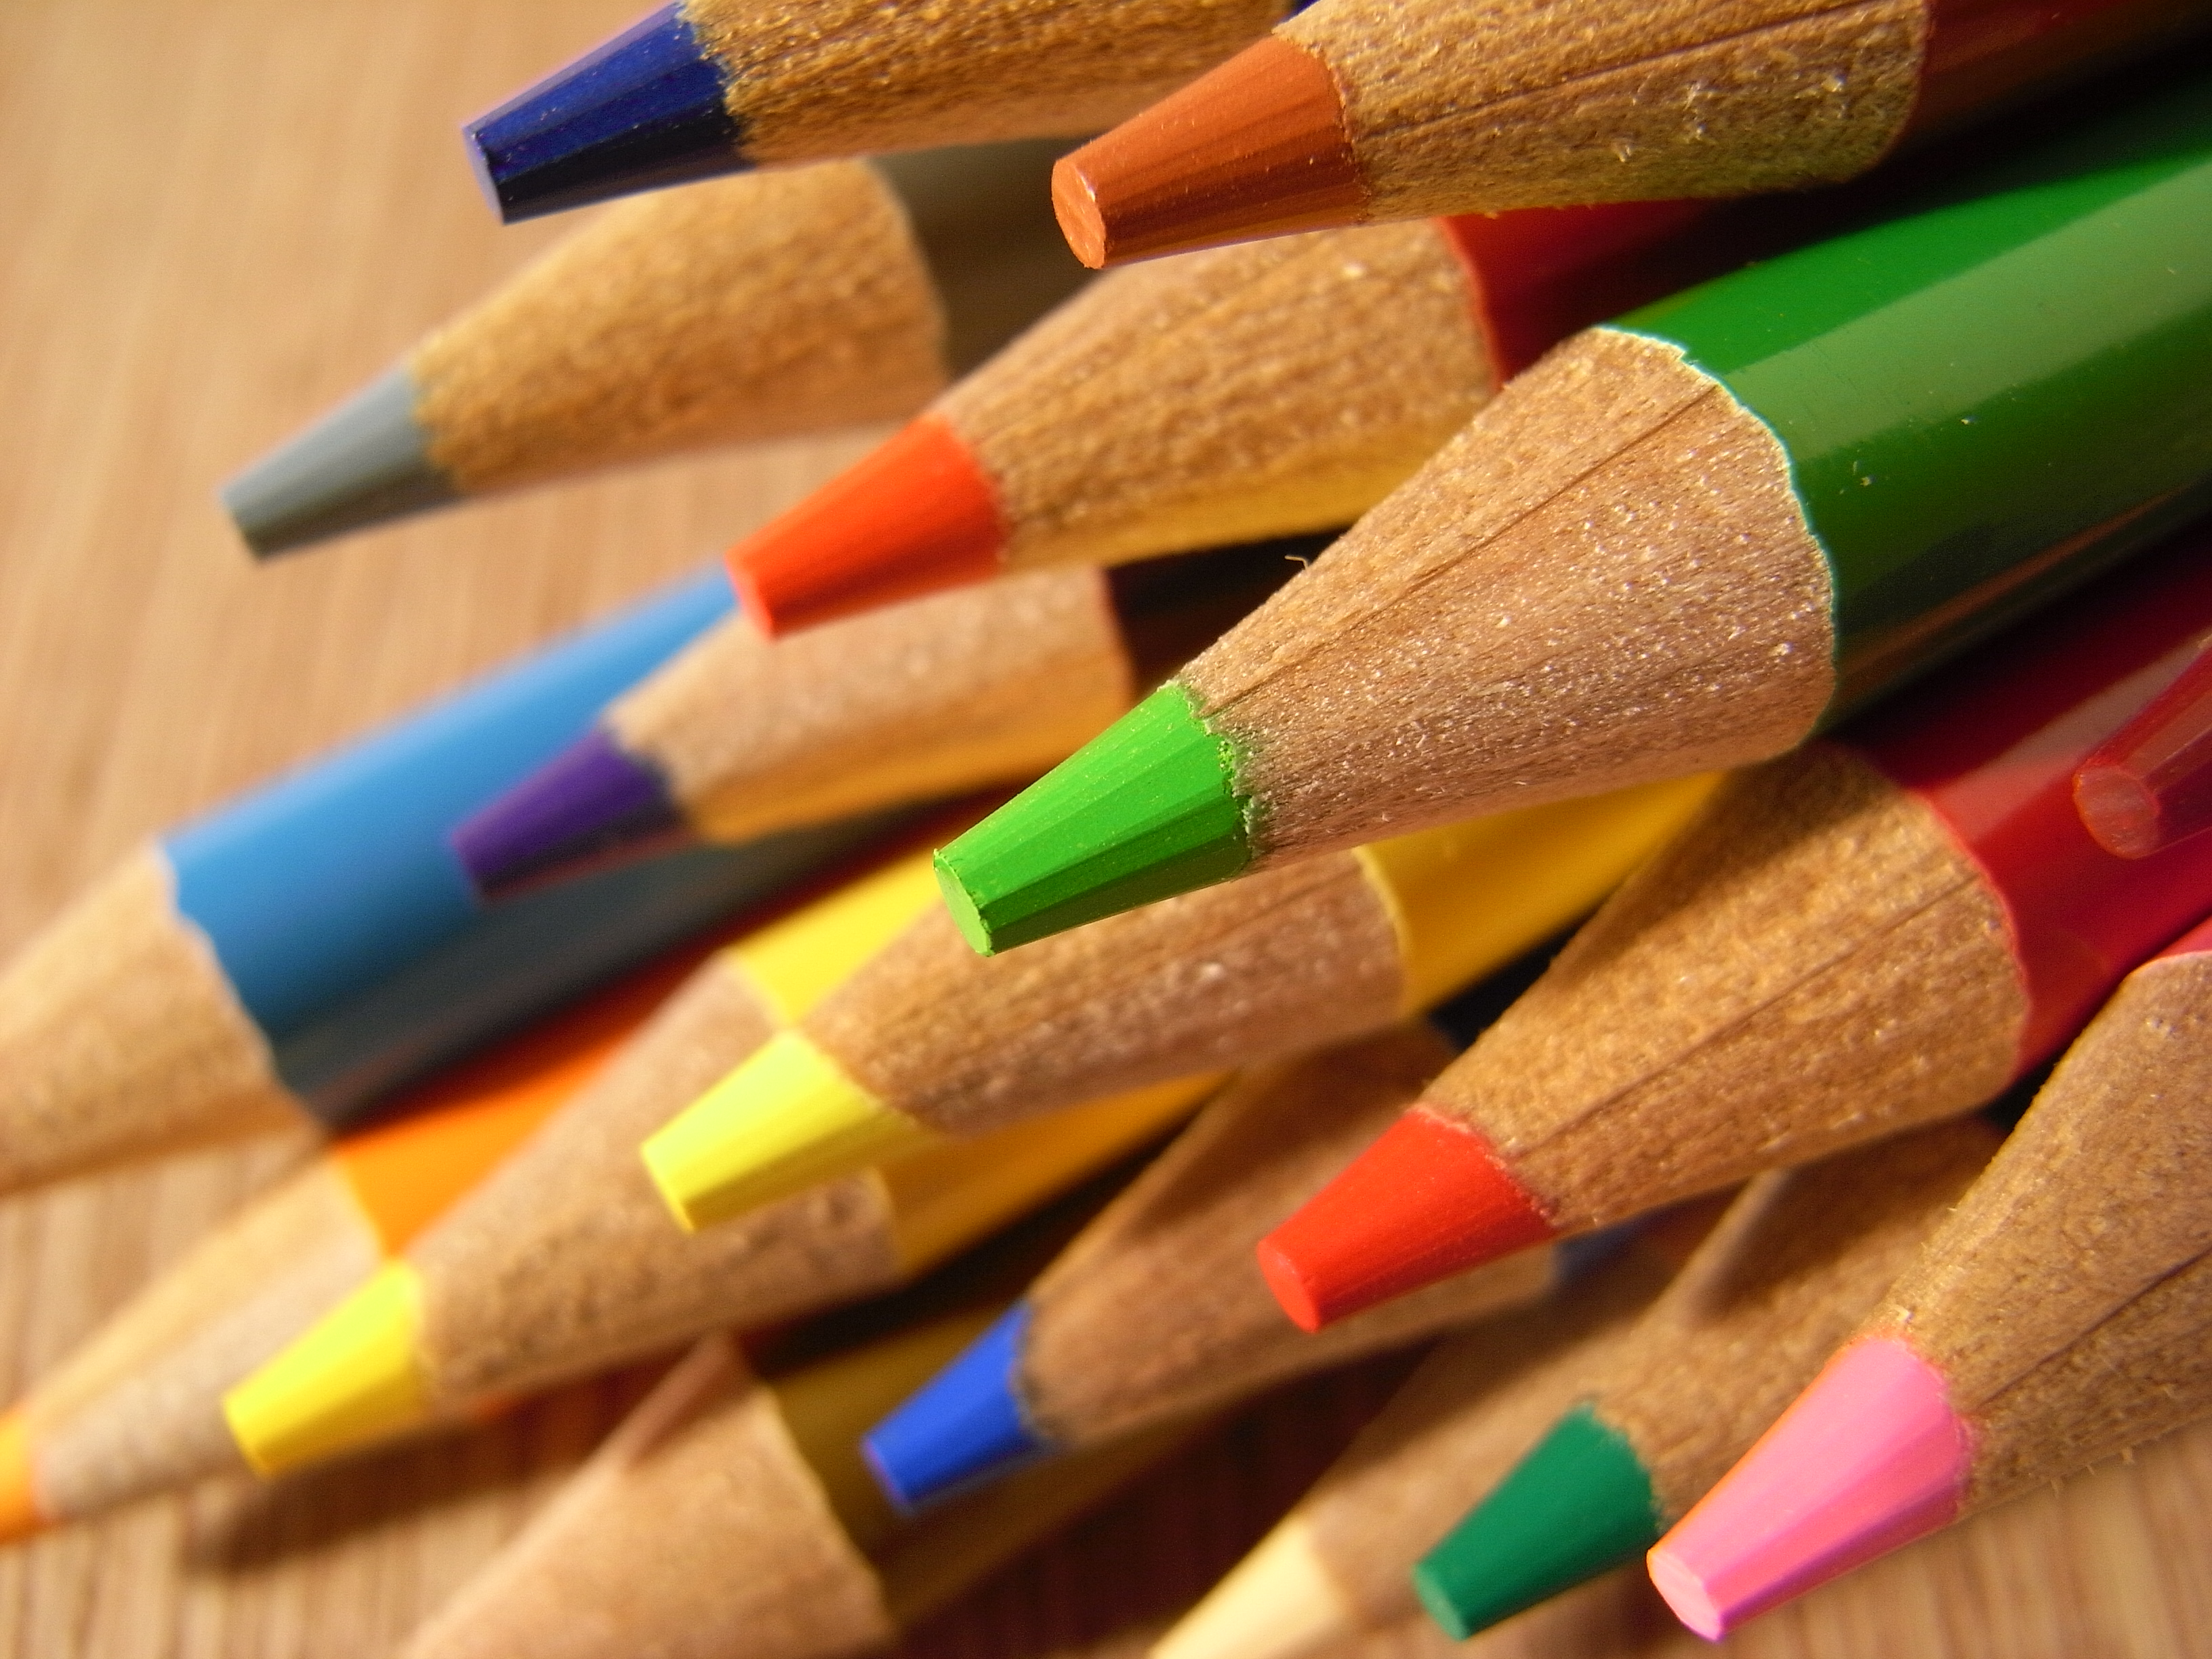
\includegraphics[width=8.5cm]{figs/chapter1/sample.jpg}
	% El que está entre corchetes va al Toc, el otro al documento
	\caption[Figura de ejemplo]{Figura de ejemplo, se incluye un texto lo suficientemente largo como para ver como queda distribuido en el documento}
	\label{fig2_intro}
\end{figure}

\lipsum[15-18]

En la Tabla \ref{table1_intro} se observan los colores disponibles.
\begin{table}[htb]
\renewcommand{\arraystretch}{1.3}
	\caption{Tabla de Colores}
	\label{table1_intro}
	\centering
	\setlength\tabcolsep{2pt}
	\begin{tabular}{c c}
		\hline
		\bfseries Código & \bfseries Color\\
		\hline
		$\mathbf{v_1}$ & Rojo\\
		$\mathbf{v_2}$ & Azul\\
		$\mathbf{v_3}$ & Verde\\
		\hline
	\end{tabular}
\end{table}

Dada la ecuación de ejemplo:
\begin{equation}
	\label{eq1_chapter1}
	E=m\,c^2
\end{equation}
Si reemplazamos $m$ en \eqref{eq1_chapter1} obtenemos la energía.

% Se agrega acá para no agregar paquetes extra al formato.
\section{Lorem Ipsum}
\lipsum[1-15]
Esto que sigue es otro footnote: \footnote{footnote number 2 working fine}